%!TEX TS-program = pdflatex

\documentclass[a4paper,11pt,twoside=semi]{scrreprt}
\usepackage[utf8]{inputenc}
\usepackage[english]{babel}
\usepackage[pdftex]{graphicx}
\graphicspath{{./fig/}}
\DeclareGraphicsExtensions{.pdf,.jpeg,.png}
\usepackage{hyperref}
\usepackage{mdframed}
\usepackage[margin=3cm]{geometry}
\usepackage[automark,headsepline]{scrlayer-scrpage}

\clearpairofpagestyles
\cfoot[\pagemark]{\pagemark}
\lehead{\headmark}
\rohead{\headmark}
\pagestyle{scrheadings}

\newcommand{\fastquote}[1]{``#1''}
\newcommand{\comment}[2]{\begin{mdframed}[backgroundcolor=yellow]\footnotesize \textbf{#1} (comment) \\ #2 \end{mdframed}}
\newcommand{\todo}[2]{\begin{mdframed}[backgroundcolor=red]\footnotesize \textbf{TODO $\rightarrow$ #1:} #2 \end{mdframed}}

\setlength{\parskip}{0.3cm}

\title{OpenState Specification}
\subtitle{Version 1.0 (beta)}
\author{}
\date{June 2015}


\begin{document}

\maketitle

\pagenumbering{Roman}

\tableofcontents

\newpage
\clearpage


\pagenumbering{arabic}

%!TEX root=main.tex

\chapter{Introduction}

\todo{Carmelo}{This section should give a clue of what OpenState is to someone who is at least confortable to the OpenFlow specification}

This document describes an extension to the OpenFlow specification v1.x () to enable support to stateful packet forwarding inside OpenFlow-enabled switches. Backward compatibility with OpenFlow is always guaranteed an exisitng elements and primitives are not modified in a way that breaks compatibility.

\begin{itemize}
	\item Motivation (Do we really need it?)
	\item Recall OpenFlow match/action flow table -> Stateless
	\item State machine abstraction
\end{itemize}



%!TEX root=000-main.tex

\chapter{Glossary}

\todo{}{}
%!TEX root=main.tex

\chapter{Stateful Pipeline}

% Difference between stateless/stateful stage
As defined by the OpenFlow specification, a packet entering an OpenFlow switch is processed through a pipeline comprised of a set of linked flow tables that provide matching, forwarding, and packet modification. We indicate with the term \emph{stateless stage} the processing operated by a single stateless OpenFlow's flow table. Conversely, we define as \emph{stateful stage} (Figure~\ref{f:stateful-stage}) a logical stage comprising a state table and and a flow table, and implementing our abstraction.

\begin{figure}[h]
	\centering
	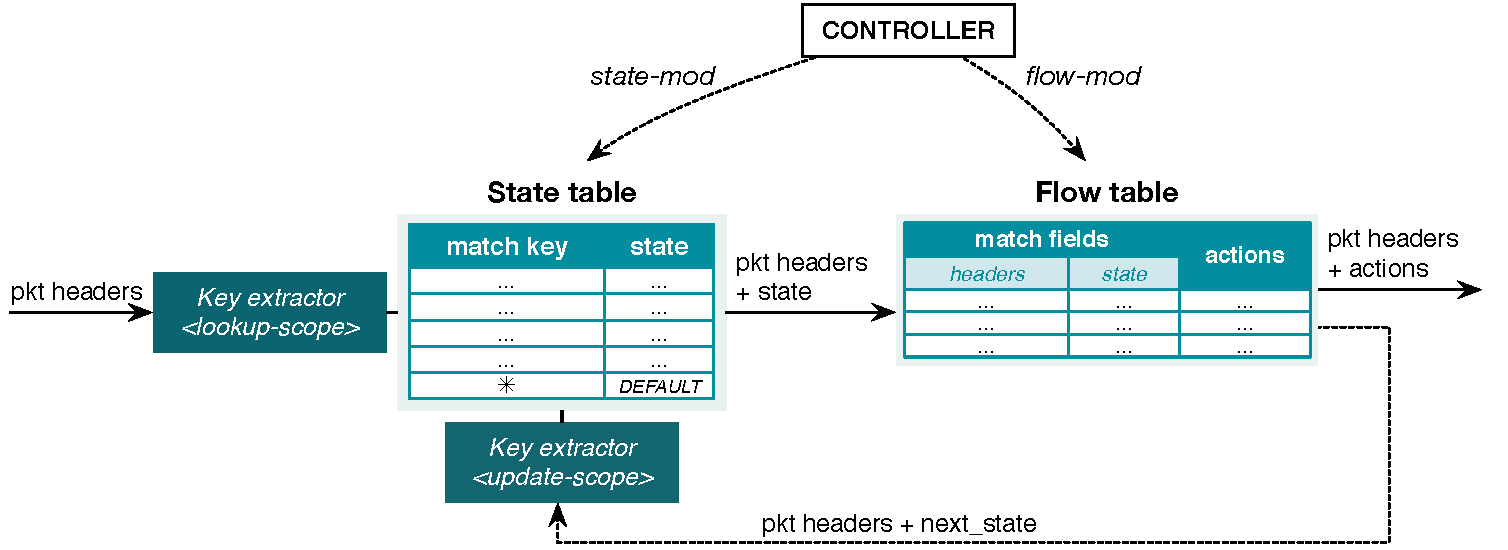
\includegraphics[width=\textwidth]{stateful-stage-arch}
	\caption{Architecture of an OpenState stateful stage}
	\label{f:stateful-stage}
\end{figure}

When a packet enters a stateful stage, it is first processed by a \emph{key extractor} which produces a string of bits representing the key to be used to match a row in the state table. The key is derived by concatenating the header fields defined in the \emph{lookup-scope}. The matched state label is appended to the packet headers as an additional header field. In case of a table-miss (the key is not matched) then a \emph{DEFAULT} state will be appended to the packet headers. If the header fields specified by the lookup-scope are not found (e.g. extracting the IP source address when the Ethernet type is not IP), a special state value \emph{NULL} is returned. By exiting the state table, packet headers along with the returned state label are matched in the flow table.

The flow table is extended by adding support to a new ``state'' virtual header field to be used to match packets along with classic header fields (MPLS, IP, TCP, etc.). We say this header is virtual because it is not really appended to the packet header and it is valid only for current processing trough the flow table of the stateful stage. Moreover a new set-state action is introduced to allow to update the state value for a given flow in a given stateful stage. The set-state action can be called as any other OpenFlow action.

\comment{Carmelo}{Is it correct to say that state labels are valid only inside the stateful stage that produced them? In other words, can I match on multiple state labels provided by different stateful stages?}

\comment{Luca e Davide}{@Carmelo: It is correct! A state label can be matched only inside the stage that produced it. In a flow entry is not possible to match over multiple state fields, but it is possible to think a distributed match over multiple stages. For example, it is possible to match over a state defined in stage 1 and then, by using the metadata field to take into account the precedent match, you can process the packet in the stage 2 to match over another state. In this way you have matched over states defined in stage 1 and stage 2}

By default all the flow tables in the switch are intended as stateless stages, the controller can then enable stateful processing for one or more stages by sending a special control message to the switch and by configuring the key extractors (lookup-scope and update-scope) associated with the state table. Similarly to flow tables, new modification message called \emph{state-mod} has been defined to allow the controller to configure the state entries and key extractors.


\todo{Carmelo}{
	\begin{itemize}
		\item Global-states introduction
	\end{itemize}
}


%A new switch capability has been defined in order to support all the OpenState functionalities, namely flow-states and global-states. A new state modify message called \emph{state-mod} has been defined to allow the controller to configure the state entries and key extractors. Finally two new actions \textbf{set-state} and \textbf{set-flags} have been defined in order to respectively implement and configure the XFSM state transitions in the flow table and set the global states.
%!TEX root=000-main.tex

\chapter{Flow States}
\label{chap:flow_states}

\todo{??}{Refactoring. This section should contain an high level description of the necessary elements and primitives to handle flow states, no C struct nor protocol message specification should be given here. These should be included in the protocol section along with checks and errors.}

A flow-state is an information associated to a flow and shared among all the flow's packets. Flows are uniquelly defined by the lookup-scope and update-scope. TBC.

\section{State Table}

\todo{??}{

Describe the state table in terms of:
    \begin{itemize}
        \item columns (key, state label, timeouts, counters?)
        \item exact match
        \item table-miss (DEFAULT vs NULL)
        \item timeouts
    \end{itemize}
}

In case of table-miss (the key is not matched) then a \texttt{DEFAULT} state will be appended to the packet headers.

\subsection{Key Extractor}

\todo{??}{
Describe the key extractor in terms of:
    \begin{itemize}
        \item difference between lookup/update (we should discuss, see next comment)
        \item vector of header fields
        \item header-miss (what if the specified header doesn't exist)
    \end{itemize}
}

\comment{Carmelo}{It seems that the only case where I need to declare two distinct lookup-scope/update-scope is when I need to update the state for the reverse flow (e.g. MAC learning, reverse path forwarding consistency, etc.). Would it be better to define just one flow-scope (essentially the lookup scope) and give the possibility to call a set-state on a transformation of this flow scope? Example: I define the flow-scope as f=\{ipsrc,ipdst\} and I define a reverse() function, that returns the definition of the reverse flow for the passed scope. In this case it would be reverse(f) = \{ipdst,ipsrc\} }

If the header fields specified by the lookup-scope are not found (e.g. extracting the IP source address when the Ethernet type is not IP) or are only partially found, a special state value \texttt{NULL} is returned and no information about state is appended to the packet.

\section{Set-state Action}
\label{sec:act_set_state}

The \texttt{OFPAT\_SET\_STATE} action allows to set flow-states in a particulare stage of the pipeline.

The structure of the \texttt{OFPAT\_SET\_STATE} is defined in the following:

\begin{verbatim}
/* Action structure for OFPAT_SET_STATE. */
struct ofp_action_set_state {
    uint16_t type;     /* OFPAT_SET_STATE */
    uint16_t len;      /* Length is 16. */
    uint32_t state;    /* State value. */
    uint8_t stage_id;  /* Stage ID (same as flow table ID) of the state table */
    uint8_t pad[7];    /* Align to 64-bits. */
};
OFP_ASSERT(sizeof(struct ofp_action_set_state) == 16);
\end{verbatim}

\comment{Carmelo}{I think we should rename stage\_id into table\_id for consistency with the OpenFlow specification}
\comment{Luca, Davide}{\textbf{To Carmelo:} Since a stateful stage comprises a state table and and a flow table, we used stage\_id because we are not referring to the single flow table (table\_id) but we are referring to the entire stateful stage. }

\subsection{Atomicity}
As defined in OpenFlow, actions are usually executed at the end of the pipeline. The same applies for the \textbf{set-state} action, thus making the stateful steps ``lookup/update'' not atomic by default. Not enforcing atomicity can bring to consistency issues when more than one packet are processed by the pipeline at the same time. The only way to guarantees state consistency between packets is to call the \textbf{set-state} action from the \textbf{apply-action} instruction (instead of the \textbf{write-actions} instruction) in order to be sure to update the value contained in the state table when exiting a specific stage of the pipeline.

\subsection{Checks and Errors}

\begin{itemize}
\item Set-state action can be called only on stateful stage. This check is performed at action execution time (maybe the flow-mod message with a set-state action is received by the switch before configuring a stage as stateful. The important thing is that the stage is stateful at action execution time).
\comment{Luca, Davide}{Should we inform the controller about this error?}

\item Set-state action must be performed onto a stage with \texttt{stage\_id} less or equal than the number of pipeline’s tables. This check is performed at msg unpack time (the number of table is fixed, so installing a flow with a wrong action does not make sense). \todo{Luca, Davide}{}
\end{itemize}

\subsection{Priority}

The new \texttt{OFPAT\_SET\_STATE} action has to be executed with an higher priority with respect to the \texttt{OFPAT\_SET\_FIELD} action. Given an action set containing both a set field and a set state action, with this setting it is avoided that the set field modifies header fields used by the set state's update scope before the set state execution.

\comment{Carmelo}{What's the priority with regards to other actions such as output, drop, etc? I think we should explain this.}

\subsection{State Match Field}
\label{sec:match_state}

The \texttt{OXM\_OF\_STATE} field is the field used in the flow table to match on the state value defined in the virtual packet header field returned by a state table in a stateful stage. It is a 32 bit field.

\comment{Luca, Davide}{Does OXM\_OF\_STATE need to have a mask?}
\comment{Carmelo}{\textbf{To Luca, Davide:} I think yes, the state field should be maskable. An example use case could be matching on the second half of a MPLS label describing the ingress/egress switch. In the same way I propose to introduce the possibility to mask the state value in the set-state action.}

\begin{verbatim}
/* Flow state field definition (oxm-match.h) */
#define OXM_OF_STATE OXM_HEADER     (0x8000, 41, 4)
\end{verbatim}

\section{State Modification Messages}
\label{sec:msg_set_state}

OpenState defines four different types of \texttt{OFPT\_STATE\_MOD} messages: 
\begin{itemize}
\setlength\itemsep{0em}
\item \textbf{Set-lookup-extractor}: allows the controller to set the vector of header fields of the lookup-scope;
\item \textbf{Set-update-extractor}: allows the controller to set the vector of header fields of the update-scope;
\item \textbf{Set-flow-state command}: allows the controller to add/update a new row in the state table (equivalent to the set-state action);
\item \textbf{Delete-flow-state}: allows the controller to delete a row in the state table (equivalent to invoking a  set-flow-state command or a set-state action with \texttt{DEFAULT} state).
\end{itemize}

The structures used

\begin{verbatim}
/*
 * Controller to switch message  (add to enum ofp_type)
 */
OFPT_STATE_MOD = 30

/*
 * Max number of fields that can be used to compose
 * the key extractor vector.
 */
#define OFPSC_MAX_FIELD_COUNT 6

/*
 * Number of bytes composing the state key
 */
#define OFPSC_MAX_KEY_LEN 48


struct ofp_state_mod {
    struct   ofp_header header;
    uint64_t cookie;
    uint64_t cookie_mask;
    uint8_t  table_id;
    uint8_t  command;
    uint8_t  payload[];
};
\end{verbatim}

\comment{Luca, Davide}{
From OpenFlow spec:
\textit{The cookie field is an opaque data value chosen by the controller. This value appears in flow removed
messages and flow statistics, and can also be used to filter flow statistics, flow modification and flow deletion. It is not used by the packet processing pipeline. When a flow entry is inserted in a table through an OFPFC\_ADD message, its cookie field is set to the provided value. When a flow entry is modified (OFPFC\_MODIFY or OFPFC\_MODIFY\_STRICT messages), its cookie field is unchanged.}

Why has it been included in the ofp\_state\_mod message?
}

\begin{verbatim}
struct ofp_state_entry {
    uint32_t key_len;
    uint32_t state;
    uint8_t  key[OFPSC_MAX_KEY_LEN];
};

struct ofp_extraction {
    uint32_t field_count;
    uint32_t fields[OFPSC_MAX_FIELD_COUNT];
};

enum ofp_state_mod_command {
	OFPSC_SET_L_EXTRACTOR = 0,
	OFPSC_SET_U_EXTRACTOR,
	OFPSC_ADD_FLOW_STATE,	
	OFPSC_DEL_FLOW_STATE
 };

\end{verbatim}

\comment{Carmelo}{enum values are not defined for ofp\_state\_mod\_command}

\comment{Luca, Davide}{\textbf{To Carmelo:} An enumerator with no = defines its value by adding 1 to the value of the previous enumeration constant }

\comment{Luca, Davide}{who decides OFPSC\_MAX\_FIELD\_COUNT and OFPSC\_MAX\_KEY\_LEN? Should they be configurable?}

\subsubsection{Set-lookup-extractor command}
\label{subsec:set_l_extr}

The \texttt{OFPSC\_SET\_L\_EXTRACTOR} command gives the opportunity to set the lookup scope used in the state table.
The controller sends a \texttt{OFPT\_STATE\_MOD} message with the following parameters:

\begin{itemize}
\item table\_id = ID of the stage to be setup
\item command = 0 (\texttt{OFPSC\_SET\_L\_EXTRACTOR})
\item field\_count = number of specified field 
\item fields = key’s fields
\end{itemize}

\todo{Luca, Davide}{Include C struct of OFPSC\_SET\_L\_EXTRACTOR}
\comment{Luca, Davide}{A Set-lookup-extractor command is a ofp\_state\_mod message with command = 0 and struct ofp\_extraction as ofp\_state\_mod's payload}

\subsubsection{Set-update-extractor command}
\label{subsec:set_u_extr}

The OFPSC\_SET\_U\_EXTRACTOR command gives the opportunity to set the update scope used in the state table.
The controller sends a \texttt{OFPT\_STATE\_MOD} message with the following parameters:

\begin{itemize}
\item table\_id = ID of the stage to be setup
\item command = 1 (OFPSC\_SET\_U\_EXTRACTOR)
\item field\_count = number of specified field 
\item fields = key’s fields
\end{itemize}

\todo{Luca, Davide}{Include C struct of OFPSC\_SET\_U\_EXTRACTOR}
\comment{Luca, Davide}{A Set-update-extractor command is a ofp\_state\_mod message with command = 1 and struct ofp\_extraction as ofp\_state\_mod's payload}

\subsection{Set-flow-state command}
\label{subsec:add_flow}

The OFPSC\_ADD\_FLOW\_STATE command gives the opportunity to insert (or to overwrite) an entry in the state table.
The controller sends a \texttt{OFPT\_STATE\_MOD} message with the following parameters:

\begin{itemize}
\item table\_id = ID of the stage to be modified
\item command = 2 (OFPSC\_ADD\_FLOW\_STATE)
\item key\_count = it is the key size in byte
\item state = it is the state to insert in the state table
\item keys = key splitted in bytes (e.g: ip 10.0.0.1 is stored as [10,0,0,1])
\end{itemize}

\todo{Luca, Davide}{Include C struct of OFPSC\_ADD\_FLOW\_STATE}
\comment{Luca, Davide}{A Set-flow-state command is an ofp\_state\_mod message with command = 2 and struct ofp\_state\_entry as ofp\_state\_mod's payload}

\comment{Carmelo}{OFPSC\_ADD\_FLOW\_STATE should be renamed in OFPSC\_SET\_FLOW\_STATE}

\subsection{Delete-flow-state command}
\label{subsec:del_flow}

With the OFPSC\_DEL\_FLOW\_STATE command is possible to delete a state table's entry.
The controller sends a \texttt{OFPT\_STATE\_MOD} message with the following parameters:

\begin{itemize}
\item table\_id = ID of the stage to be modified
\item command = 3 (OFPSC\_DEL\_FLOW\_STATE)
\item key\_count = it is the key size in byte
\item state = ANY
\item keys = key splitted in bytes (e.g: ip 10.0.0.1 is stored as [10,0,0,1])
\end{itemize}

\todo{Luca, Davide}{Include C struct of OFPSC\_DEL\_FLOW\_STATE}
\comment{Luca, Davide}{A Delete-flow-state command is an ofp\_state\_mod message with command = 3 and struct ofp\_state\_entry as ofp\_state\_mod's payload}

The state value is not taken in consideration because the state table simply uses as key the lookup-scope's fields to delete the entry with key keys.

\paragraph{Checks and Errors}

\begin{itemize}
\item In Set-lookup-extractor/Set-update-extractor commands \texttt{field\_count} must be consistent with the number of fields provided in \texttt{fields[]}, otherwise an error (\texttt{OFPET\_BAD\_ACTION}, \texttt{OFPBAC\_BAD\_LEN}) is returned at message unpack time
\comment{Carmelo}{Are both \texttt{OFPET\_BAD\_ACTION} and \texttt{OFPBAC\_BAD\_LEN} returned?}
\comment{Luca, Davide}{\textbf{To Carmelo:} An error message has a type (\texttt{OFPET\_BAD\_ACTION}) and a code (\texttt{OFPBAC\_BAD\_LEN}): }

\item In Set-flow-state/Delete-flow-state commands \texttt{key\_count} must be consistent with the number of keys provided in \texttt{key[]}, otherwise an error (\texttt{OFPET\_BAD\_ACTION}, \texttt{OFPBAC\_BAD\_LEN}) is returned at msg unpack time. 

\item In Set-flow-state/Delete-flow-state commands \texttt{key\_count} must be consistent with the number of fields of the update-scope (defined before with a OFPSC\_SET\_U\_EXTRACTOR). This check is performed at msg execution time
\comment{Luca, Davide}{Should we inform the controller about this error?}

\item Lookup-scope and update-scope should provide same length keys. This check should be performed by the switch when a set-extractor message is received: if we have already set the other extractor, the new extractor must have the same length. The check is performed at msg execution time.
\comment{Luca, Davide}{Should we inform the controller about this error?}
\todo{Luca, Davide}

\item Set-flow-state/Delete-flow-state commands must be executed onto a stage with stage\_id less or equal than the number of pipeline’s tables, otherwise the switch returns an error (OFPET\_BAD\_REQUEST, OFPBRC\_BAD\_TABLE\_ID). This check is performed at msg unpack time (since the number of table is fixed).

\end{itemize}
%!TEX root=main.tex

\chapter{Global States}
\label{chap:global_states}
By extending the flow state concept some states could be shared among multiple flows. For this reason global states have been developed. These states (a.k.a. flags) are defined at datapath level and are not related to a single flow of a particular stage. Now each incoming flow’s packet can be matched also according to the current value of global states. Global states can be updated c by means of a new action ``set-flags'' triggered by a match in the flow table. Furthermore, the controller is able to modify and reset global states value of a specific switch exploiting the new flag modification messages.

\todo{Luca, Davide}{Decription of the global states as a string of bits, maskable. Who defines the maximum length of the string? the switch? The specification?}

\section{Flag Modification Messages}
\label{sec:flag_mod_msg}

The following types of flag modification messages are defined:

\begin{itemize}
	\item \textbf{Set-flags}: allows the controller to update the value of global states. Values can be totally overwritten or, by using a mask, selectively modified.
	\item \textbf{Reset-flags}: allows the controller to reset global states to the default value.
	\comment{Carmelo}{Who defines the default value? The switch? The controller?}
\end{itemize}

\section{Set-flag Action}
\label{sec:act_set_flag}

In addition to flag modification messages \ref{sec:flag_mod_msg}, the global states can be modified as a consequence of packet matching in a flow entry. By adding a set-flag action to the action set, it is possible to modify the global state values in any stage of the pipeline. OpenFlow allows to execute actions in the group table, so it is possible to update global state values from the group table by inserting a set-flag action in the action bucket. Using the set-flag action values can be totally overwritten or, by using a mask, selectively modified.
%!TEX root=main.tex

\chapter{Protocol}
\label{chap:protocol}

\section{Capability}
\label{sec:capability}
\scriptsize
\begin{verbatim}
OFPC_OPENSTATE = 1 << 9   /* Capabilities supported by the datapath (add to enum ofp_capabilities) */
\end{verbatim}
\normalsize
\noindent
A new \texttt{OFPC\_OPENSTATE} capability has been introduced.
The basic flow table data structure has been extended with a support data structure implementing the state table (a hash map indexed by the flow key), the lookup and update key extractor (two ordered lists of flow match TLV field indexes) and the global states.
By retrieving all the capabilities from the switch, the controller is able to properly configure the switch. If a switch is OpenState aware, the \texttt{OFPC\_OPENSTATE} capability bit is set enabling the controller to configure the statefulness of each stage by sending table feature message [\ref{sec:table_conf}].

\section{Stage Configuration}
\label{sec:table_conf}
\scriptsize
\begin{verbatim}
 OFPTC_TABLE_STATEFUL = 1 << 4   /* (add to bitmap of OFPTC_* flags) */
\end{verbatim}
\normalsize
If \texttt{OFPTC\_TABLE\_STATEFUL} bit is set in the table features' config bitmap, right after the packet headers are parsed, the flow state is retrieved and written in the state field, otherwise the packet directly jumps to the flow table. 

\section{State Modification Messages}

\label{sec:msg_set_state_proto}

Modifications to the state table from the controller are done with the \texttt{OFPT\_STATE\_MOD} message:
\scriptsize
\begin{verbatim}
OFPT_STATE_MOD = 30     /* Controller to switch message  (add to enum ofp_type) */

struct ofp_state_mod {
    struct   ofp_header header;
    uint64_t cookie;
    uint64_t cookie_mask;
    uint8_t  table_id;
    uint8_t  command;
    uint8_t  payload[];
};
\end{verbatim}
\normalsize

\comment{Luca, Davide}{
From OpenFlow spec:
\textit{The cookie field is an opaque data value chosen by the controller. This value appears in flow removed
messages and flow statistics, and can also be used to filter flow statistics, flow modification and flow deletion. It is not used by the packet processing pipeline. When a flow entry is inserted in a table through an OFPFC\_ADD message, its cookie field is set to the provided value. When a flow entry is modified (OFPFC\_MODIFY or OFPFC\_MODIFY\_STRICT messages), its cookie field is unchanged.}

Why has it been included in the ofp\_state\_mod message?
}
\noindent
The \texttt{table\_id} field specifies the table to be modified (extractors setup or states modifications).
\\\\
The \texttt{command} field must be one of the following:
\scriptsize
\begin{verbatim}
enum ofp_state_mod_command {
    OFPSC_SET_L_EXTRACTOR = 0,
    OFPSC_SET_U_EXTRACTOR,
    OFPSC_SET_FLOW_STATE,   
    OFPSC_DEL_FLOW_STATE
 };
\end{verbatim}
\normalsize
The differences between the four commands are explained in section \ref{sec:msg_set_state}.
\\\\
The \texttt{payload} field structure is defined by \texttt{ofp\_state\_entry} or \texttt{ofp\_extraction} according to the value of \texttt{command} field.
\\\\
An \texttt{OFPT\_STATE\_MOD} message with \texttt{command} field set to \texttt{OFPSC\_SET\_L\_EXTRACTOR} or \texttt{OFPSC\_SET\_U\_EXTRACTOR} must have a \texttt{payload} structure as defined by \texttt{ofp\_extraction}.
\scriptsize
\begin{verbatim}
#define OFPSC_MAX_FIELD_COUNT 6     /* Max number of fields that can be used to compose the key extractor vector*/

struct ofp_extraction {
    uint32_t field_count;
    uint32_t fields[OFPSC_MAX_FIELD_COUNT];
};
\end{verbatim}
\normalsize
The \texttt{field\_count} field specifies the number of fields provided in \texttt{fields[]}.
\\\\The \texttt{fields[]} field contains the vector of fields composing the key extractor.

\comment{Luca, Davide}{who decides OFPSC\_MAX\_FIELD\_COUNT and OFPSC\_MAX\_KEY\_LEN? Should they be configurable?}
\noindent
An \texttt{OFPT\_STATE\_MOD} message with \texttt{command} field set to \texttt{OFPSC\_SET\_FLOW\_STATE} or \texttt{OFPSC\_DEL\_FLOW\_STATE} must have a \texttt{payload} structure as defined by \texttt{ofp\_state\_entry}.
\scriptsize
\begin{verbatim}
#define OFPSC_MAX_KEY_LEN 48    /* Number of bytes composing the state key */

struct ofp_state_entry {
    uint32_t key_len;
    uint32_t state;
    uint8_t  key[OFPSC_MAX_KEY_LEN];
};
\end{verbatim}
\normalsize
The \texttt{key\_len} field specifies the number of keys provided in \texttt{key[]} (it is the key size in byte).
\\\\
The \texttt{state} field contains the state to be inserted (or updated) in the state table. In case \texttt{command} field is set to \texttt{OFPSC\_DEL\_FLOW\_STATE}, the \texttt{state} field can take any value because only \texttt{key} field is used to delete the corresponding entry in the state table.
\\\\
The \texttt{key} field contains the key used to access the state table, splitted in bytes (e.g: ip 10.0.0.1 is stored as [10,0,0,1])

\paragraph{Checks and Errors}

\begin{itemize}
\item When \texttt{command} field is set to \texttt{OFPSC\_SET\_L\_EXTRACTOR} or \texttt{OFPSC\_SET\_U\_EXTRACTOR}, \texttt{field\_count} must be consistent with the number of fields provided in \texttt{fields[]} and should be always greater than 0, otherwise the switch must return an \texttt{ofp\_error\_msg} with \texttt{OFPET\_BAD\_REQUEST} type and \texttt{OFPBRC\_BAD\_LEN} code at message unpack time.
\comment{Carmelo}{Are both \texttt{OFPET\_BAD\_ACTION} and \texttt{OFPBAC\_BAD\_LEN} returned?}
\comment{Luca, Davide}{\textbf{To Carmelo:} An error message has a type (\texttt{OFPET\_BAD\_ACTION}) and a code (\texttt{OFPBAC\_BAD\_LEN}). }

\item When \texttt{command} field is set to \texttt{OFPSC\_SET\_FLOW\_STATE} or \texttt{OFPSC\_DEL\_FLOW\_STATE}, \texttt{key\_count} field must be consistent with the number of keys provided in \texttt{key[]} and should be always greater than 0, otherwise 
the switch must return an \texttt{ofp\_error\_msg} with \texttt{OFPET\_BAD\_REQUEST} type and \texttt{OFPBRC\_BAD\_LEN} code at message unpack time.

\item When \texttt{command} field is set to \texttt{OFPSC\_SET\_FLOW\_STATE} or \texttt{OFPSC\_DEL\_FLOW\_STATE}, \texttt{key\_count} field must be consistent with the number of fields of the update-scope (previously configured with an \texttt{OFPSC\_SET\_U\_EXTRACTOR} command). This check is performed at message execution time.
\comment{Luca, Davide}{Should we inform the controller about this error?}

\item According to OpenState specifications, lookup-scope and update-scope should provide keys with same length. This check should be performed by the switch when a message with \texttt{command} field set to \texttt{OFPSC\_SET\_L\_EXTRACTOR} or \texttt{OFPSC\_SET\_U\_EXTRACTOR} is received: if the other extractor has already been configured, the new extractor key must have the same length. This check is performed at message execution time.
\comment{Luca, Davide}{Should we inform the controller about this error?}

\item When \texttt{command} field is set to \texttt{OFPSC\_SET\_FLOW\_STATE} or \texttt{OFPSC\_DEL\_FLOW\_STATE}, \texttt{table\_id} field must have a value less or equal than the number of pipeline’s tables, otherwise the switch must return an \texttt{ofp\_error\_msg} with \texttt{OFPET\_BAD\_REQUEST} type and \texttt{OFPBRC\_BAD\_TABLE\_ID} code. This check is performed at message unpack time (since the number of table is fixed).

\end{itemize}

\section{Set-state Action}
\label{sec:act_set_state_proto}

The \texttt{OFPAT\_SET\_STATE} action allows to set flow-states in a particulare stage of the pipeline.\\The following structure describes the body of set-state action:

\scriptsize
\begin{verbatim}
OFPAT_SET_STATE = 28    /* New action type  (add to enum ofp_action_type) */

/* Action structure for OFPAT_SET_STATE. */
struct ofp_action_set_state {
    uint16_t type;
    uint16_t len;
    uint32_t state;
    uint8_t table_id;
    uint8_t pad[7];    /* Align to 64-bits. */
};
OFP_ASSERT(sizeof(struct ofp_action_set_state) == 16);
\end{verbatim}
\normalsize
\noindent
The \texttt{type} field should be set to \texttt{OFPAT\_SET\_STATE}.
\\\\
The \texttt{len} field should be set to 16.
\\\\
The \texttt{state} field specifies the state to be inserted (or updated) in the state table.
\\\\
The \texttt{table\_id} field specifies the target stage of the state update action.

\subsection{Checks and Errors}

\begin{itemize}
\item Set-state action must be called only on stateful stage. This check is performed at action execution time because the flow-mod message with a set-state action could be received by the switch before configuring a stage as stateful. The important thing is that the stage is stateful at action execution time (since the number of table is fixed).
\comment{Luca, Davide}{Should we inform the controller about this error?}

\item Set-state action must be performed onto a stage with \texttt{stage\_id} less or equal than the number of pipeline’s tables, otherwise the switch must return an \texttt{ofp\_error\_msg} with \texttt{OFPET\_BAD\_REQUEST} type and \texttt{OFPBRC\_BAD\_TABLE\_ID} code. This check is performed at message unpack time (the number of table is fixed, so installing a flow with a wrong action does not make sense).
\end{itemize}

\subsection{Priority}

The actions in an action set are applied in the order specified in the OpenFlow specification, regardless of the order that
they were added to the set. The new \texttt{OFPAT\_SET\_STATE} action has to be executed with an higher priority with respect to the \texttt{OFPAT\_SET\_FIELD} action. Given an action set containing both a set field and a set state action, with this setting it is avoided that the set field modifies header fields used by the set state's update scope before the set-state action execution.

\comment{Carmelo}{What's the priority with regards to other actions such as output, drop, etc? I think we should explain this.}
\comment{Luca,Davide}{Assumption: we want to perform set-state action before some other action of the same stage alters its header fields. For example the pop/push actions could modify it. So, in order to avoid it, we should define the highest possible priority for the set-state action.
Is the assumption legitimate?
\\ What if we set the highest possible priority and we want to perform a set-state action on a packet modified by other actions? We would need two stages: the first modifies header fields and the other executes the set-state action.
}

\section{State Match Field}
\label{sec:match_state}

The \texttt{OXM\_OF\_STATE} field is the field used in the flow table to match on the state value defined in the virtual packet header field returned by a state table in a stateful stage. It is a 32 bit field.

\comment{Luca, Davide}{Does OXM\_OF\_STATE need to have a mask?}
\comment{Carmelo}{\textbf{To Luca, Davide:} I think yes, the state field should be maskable. An example use case could be matching on the second half of a MPLS label describing the ingress/egress switch. In the same way I propose to introduce the possibility to mask the state value in the set-state action.}
\scriptsize
\begin{verbatim}
/* Flow state field definition (oxm-match.h) */
#define OXM_OF_STATE OXM_HEADER     (0x8000, 41, 4)
\end{verbatim}
\normalsize

\section{Flag modification messages}
\label{sec:flag_mod_msg_proto}
Modifications to the global states from the controller are done with the \texttt{OFPT\_FLAG\_MOD} message.

\scriptsize\begin{verbatim}
OFPT_FLAG_MOD = 31,  /* Controller/switch message */

struct ofp_flag_mod {
    struct ofp_header header;
    uint32_t flag;
    uint32_t flag_mask;
    uint8_t command;
    uint8_t pad[7];                  /* Pad to 64 bits. */
};
\end{verbatim}\normalsize

\noindent
The \texttt{flag} field specifies the new value of global states.
\\\\The \texttt{flag\_mask} field specifies which bits of the global state should be modified. A \texttt{flag\_mask} with value \texttt{0xFFFFFFFFFFFFFFFF} indicates that the global state field should be entirely overwritten.
The \texttt{command} field must be one of the following:

\scriptsize\begin{verbatim}
enum ofp_flag_mod_command { 
    OFPSC_MODIFY_FLAGS = 0,
    OFPSC_RESET_FLAGS
};
\end{verbatim}\normalsize
\noindent
The differences between the two commands are explained in section \ref{sec:flag_mod_msg}.

\scriptsize\begin{verbatim}
#define OFP_GLOBAL_STATES_DEFAULT 0
\end{verbatim}\normalsize
\noindent
In case command field is set to \texttt{OFPSC\_RESET\_FLAGS}, both the \texttt{flag} field and the \texttt{flag\_mask} can take any value and global states are reset to the default value defined in \texttt{OFP\_GLOBAL\_STATES\_DEFAULT}.

\comment{Luca e Davide}{Does the OFP\_GLOBAL\_STATES\_DEFAULT be configurable?}



\section{Set-flag action}
\label{sec:set_flag_action_proto}
The \texttt{OFPAT\_SET\_FLAG} action is used to set flags' value.
The following structure describes the body of set-flag action:

\scriptsize\begin{verbatim}
OFPAT_SET_FLAG = 29,   /* Set a single flag value of the global state */

/* Action structure for OFPAT_SET_FLAG */
struct ofp_action_set_flag {
    uint16_t type;
    uint16_t len; 
    uint32_t flag;
    uint32_t flag_mask;   
    uint8_t pad[4];   /* Align to 64-bits. */
};
OFP_ASSERT(sizeof(struct ofp_action_set_flag) == 16);
\end{verbatim}\normalsize

\noindent
The \texttt{type} field should be set to \texttt{OFPAT\_SET\_FLAG}.
\\\\
The \texttt{len} field should be set to 16.
\\\\
The \texttt{value} field specifies the new value of global states.
\\\\
The \texttt{flag} field specifies which bits of the global state should be modified. A \texttt{flag\_mask} with value \texttt{0xFFFFFFFFFFFFFFFF} indicates that the global state field should be entirely overwritten.

\section{Flags match field}
\label{section:oxm_of_flags}

If a switch supports OpenState (capability OFPC\_OPENSTATE), right after the packet headers are parsed, the global states are retrieved and written in the flags field. OXM\_OF\_FLAGS is a field with mask, so it is possible to match it either exactly or with wildcards. A 0 bit in the mask means i-th flags value is ``do not care'', while a 1 bit value means ``exact match''.

\scriptsize\begin{verbatim}
/* Global States */
#define OXM_OF_FLAGS OXM_HEADER     (0x8000, 40, 4)
#define OXM_OF_FLAGS_W OXM_HEADER_W (0x8000, 40, 4)
\end{verbatim}\normalsize
Example match:
\scriptsize\begin{verbatim}
flags=(4,5)
\end{verbatim}\normalsize
This command allows to match over *****************************1*0 flags configuration (4 in binary is 100 and the mask 5 is 101 that is exact match on LSB 1 (0 value) and LSB 3 (1 value) and ``don’t care'' over all the other flags. In order to perform an exact match on flags value no mask is required.
\\Example match:
\scriptsize\begin{verbatim}
flags=4
\end{verbatim}\normalsize
NB: this match is very differend from the previous one. With this command we are matching over 00000000000000000000000000000100 flags configuration, so it is an exact match.



\section*{Credits}
Spec contributions, in alphabetical order: Giuseppe Bianchi, Marco Bonola, Antonio Capone, Carmelo Cascone, Luca Pollini, Davide Sanvito


\end{document}

